\documentclass{beamer}

% Packages
\usepackage[utf8]{inputenc}
\usepackage{graphicx}
\usepackage{amsmath}
\usepackage{booktabs}
\usepackage{hyperref}
\usepackage{caption}

% Title Page
\title{Développement d'un modèle de scoring crédit pour Prêt à dépenser}
\author{Antoine Fusilier}
\institute{Prêt à dépenser}
\date{\today}

\begin{document}
\small
% Title Slide
\begin{frame}
    \titlepage
\end{frame}

% Slide 1: Introduction
\begin{frame}{Introduction}
    \begin{itemize}
        \item \textbf{Importance du scoring crédit} : Le scoring crédit est essentiel pour les institutions financières, permettant de minimiser les risques liés aux défauts de paiement tout en optimisant les opportunités de prêt.
        \item \textbf{Défis associés} : Interprétabilité, gestion du déséquilibre des classes, et minimisation des coûts d'erreurs.
        \item \textbf{Impact sur l'entreprise} : Un modèle efficace réduit les pertes financières, améliore la satisfaction client, et renforce la compétitivité de "Prêt à dépenser".
    \end{itemize}
\end{frame}

% Slide 2: Description des données
\begin{frame}{Description des données}
    \begin{itemize}
        \item \textbf{Source des données} : Historique des prêts, informations financières des clients, et leur comportement de paiement.
        \item \textbf{Exploration des données} :
            \begin{itemize}
                \item \textbf{Analyse des distributions} : Identifier les variables avec des distributions asymétriques ou des outliers.
                \item \textbf{Matrice de corrélation} : Détecter les relations linéaires pour éviter la multicolinéarité.
                \item \textbf{Formule de corrélation} :
                \[
                \text{Corrélation} = \frac{\text{Cov}(X, Y)}{\sigma_X \sigma_Y}
                \]
            \end{itemize}
        \item \textbf{Insights clés} : Les variables liées au revenu et à l'endettement montrent une forte corrélation avec les défauts de paiement.
    \end{itemize}
    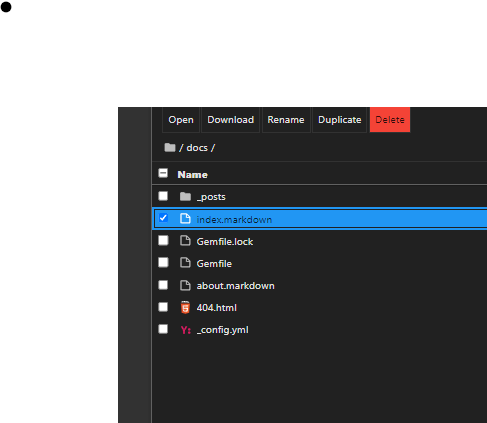
\includegraphics[width=\textwidth]{assets/test.png} % Remplacer par le chemin de l'image
\end{frame}

% Slide 3: Nettoyage des données
\begin{frame}{Nettoyage des données}
    \begin{itemize}
        \item \textbf{Gestion des valeurs manquantes} :
            \begin{itemize}
                \item \textbf{Méthode d'imputation} : Imputation par la médiane pour les variables continues, par la mode pour les catégorielles.
                \item \textbf{Méthodes avancées} : Imputation avec KNN pour conserver les relations entre variables.
                \item \textbf{Impact sur le modèle} : L'imputation correcte des données manquantes améliore la robustesse du modèle.
            \end{itemize}
        \item \textbf{Traitement des outliers} :
            \begin{itemize}
                \item \textbf{Identification} : Utilisation de l'Isolation Forest pour détecter les anomalies dans les données.
                \item \textbf{Méthode} : Transformation logarithmique pour les variables à distribution asymétrique.
                \item \textbf{Formule d'Isolation Forest} :
                \[
                \text{Score} = 2^{-\frac{\text{distance}}{\text{average path length}}}
                \]
                \item \textbf{Conséquences} : Les outliers peuvent biaiser le modèle; leur traitement est donc essentiel pour des prédictions précises.
            \end{itemize}
        \item \textbf{Normalisation des données} :
            \begin{itemize}
                \item Utilisation du Z-score pour standardiser les variables :
                \[
                \text{Z-score} = \frac{X - \mu}{\sigma}
                \]
                \item \textbf{Pourquoi ?} : Les modèles basés sur la distance, comme KNN ou SVM, nécessitent des données normalisées pour une performance optimale.
            \end{itemize}
    \end{itemize}
    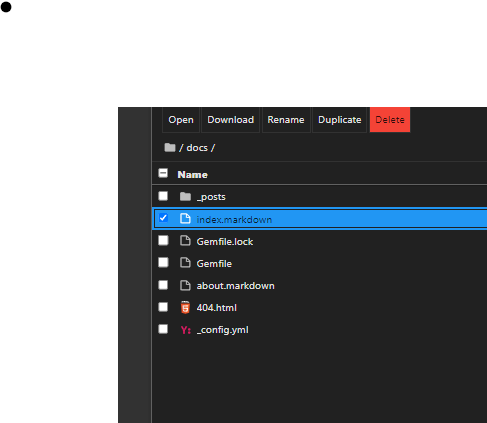
\includegraphics[width=\textwidth]{assets/test.png} % Remplacer par le chemin de l'image
\end{frame}

% Slide 4: Feature Engineering
\begin{frame}{Feature Engineering}
    \begin{itemize}
        \item \textbf{Création de nouvelles variables} :
            \begin{itemize}
                \item \textbf{Exemples} : Ratio dette/revenu, score d'endettement basé sur l'historique.
                \item \textbf{Justification} : Les nouvelles variables capturent des informations critiques qui ne sont pas directement présentes dans les données brutes.
                \item \textbf{Impact attendu} : Amélioration significative de la capacité prédictive du modèle.
            \end{itemize}
        \item \textbf{Encodage des variables catégorielles} :
            \begin{itemize}
                \item \textbf{Techniques utilisées} : One-Hot Encoding pour les variables sans ordre, Target Encoding pour les variables avec influence sur la cible.
                \item \textbf{Risques} : Sur-ajustement possible avec Target Encoding, nécessitant une validation croisée rigoureuse.
            \end{itemize}
        \item \textbf{Sélection des variables} :
            \begin{itemize}
                \item \textbf{Méthodes} : PCA pour la réduction de dimensionnalité, analyse de variance pour identifier les variables pertinentes.
                \item \textbf{Pourquoi ?} : Réduire la complexité du modèle tout en conservant l'information pertinente.
            \end{itemize}
    \end{itemize}
    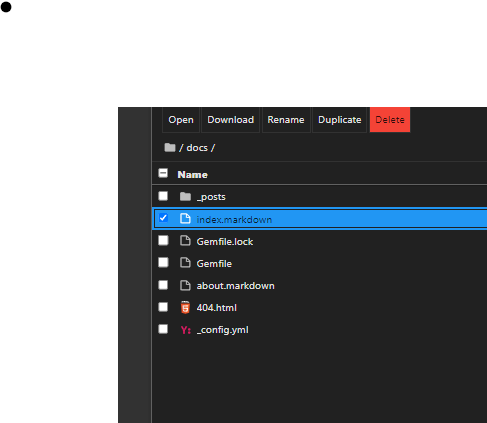
\includegraphics[width=\textwidth]{assets/test.png} % Remplacer par le chemin de l'image
\end{frame}

% Slide 5: Modélisation
\begin{frame}{Modélisation}
    \begin{itemize}
        \item \textbf{Algorithmes testés} :
            \begin{itemize}
                \item \textbf{Régression Logistique} :
                \[
                \hat{y} = \frac{1}{1 + e^{-(\beta_0 + \beta_1 X_1 + \dots + \beta_n X_n)}}
                \]
                \item \textbf{Random Forest} :
                \[
                \text{Prediction} = \frac{1}{N} \sum_{i=1}^{N} f_i(x)
                \]
                \item \textbf{XGBoost} :
                \[
                \text{Obj}(\theta) = \sum_{i=1}^{n} l(y_i, \hat{y}_i) + \sum_{j=1}^{k} \Omega(f_j)
                \]
                \item \textbf{LightGBM} :
                \[
                \text{Split Gain} = \left[\frac{G_L^2}{H_L + \lambda} + \frac{G_R^2}{H_R + \lambda} - \frac{(G_L + G_R)^2}{H_L + H_R + \lambda}\right] - \gamma
                \]
            \end{itemize}
        \item \textbf{Validation croisée} :
            \begin{itemize}
                \item Cross-Validation avec GridSearchCV pour l'optimisation des hyperparamètres.
                \item \textbf{Pourquoi ?} : Éviter l'overfitting et sélectionner le meilleur modèle pour la généralisation.
            \end{itemize}
        \item \textbf{Interprétation des résultats} :
            \begin{itemize}
                \item \textbf{Comparaison des modèles} : Régression logistique pour l'interprétabilité, XGBoost pour la performance.
                \item \textbf{Choix final} : LightGBM pour son équilibre entre performance et efficacité.
            \end{itemize}
    \end{itemize}
    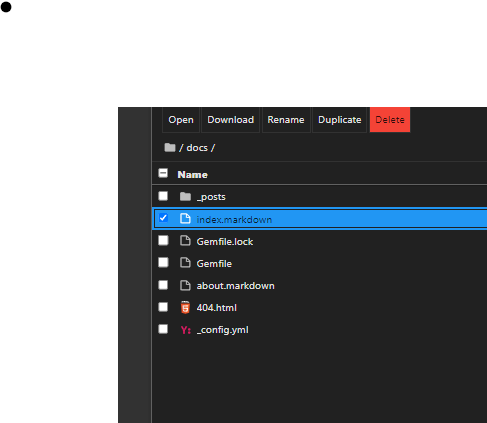
\includegraphics[width=\textwidth]{assets/test.png} % Remplacer par le chemin de l'image
\end{frame}

% Slide 6: Comparaison des modèles
\begin{frame}{Comparaison des modèles}
    \begin{table}[]
        \centering
        \caption{Comparaison des modèles testés}
        \begin{tabular}{@{}lcccc@{}}
        \toprule
        \textbf{Modèle} & \textbf{AUC} & \textbf{Accuracy} & \textbf{F1-Score} & \textbf{Score métier} \\ \midrule
        Régression Logistique & 0.75 & 0.70 & 0.65 & 0.68 \\
        Random Forest & 0.80 & 0.75 & 0.72 & 0.74 \\
        XGBoost & 0.82 & 0.77 & 0.74 & 0.78 \\
        LightGBM & 0.83 & 0.78 & 0.75 & 0.80 \\
        SVM & 0.77 & 0.72 & 0.68 & 0.70 \\ \bottomrule
        \end{tabular}
    \end{table}
    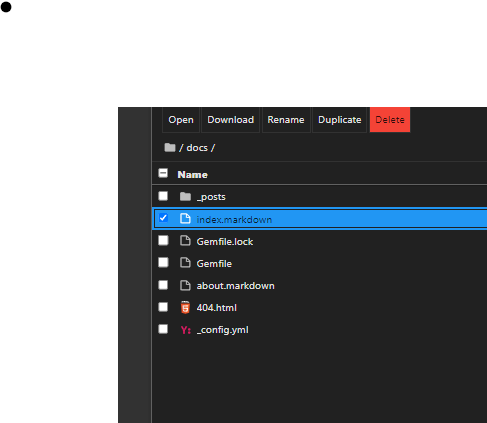
\includegraphics[width=\textwidth]{assets/test.png} % Remplacer par le chemin de l'image
    \captionof{figure}{Comparaison des courbes ROC des modèles testés}
\end{frame}

% Slide 7: Résultats des Modèles
\begin{frame}{Résultats des Modèles}
    \begin{itemize}
        \item \textbf{Meilleur modèle retenu} : LightGBM
        \item \textbf{Performance} :
            \begin{itemize}
                \item AUC: 0.83
                \item Accuracy: 0.78
                \item F1-Score: 0.75
                \item Score métier: 0.80
            \end{itemize}
        \item \textbf{Optimisation du seuil} : Ajustement du seuil de décision pour minimiser les coûts liés aux erreurs FN et FP.
        \[
        \text{Score Métier} = \text{minimiser le coût} = FN \times 10 + FP
        \]
        \item \textbf{Implication} : Ce modèle offre un bon compromis entre précision et minimisation des coûts.
    \end{itemize}
    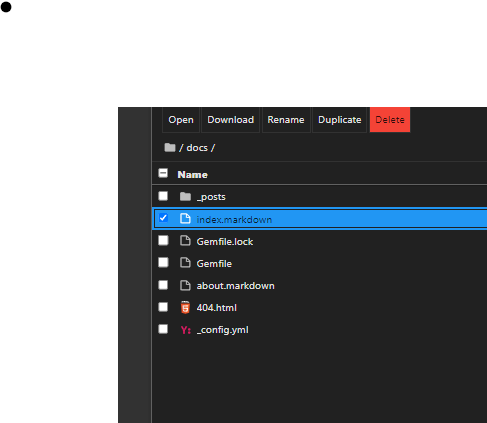
\includegraphics[width=\textwidth]{assets/test.png} % Remplacer par le chemin de l'image
\end{frame}

% Slide 8: Interprétabilité du Modèle
\begin{frame}{Interprétabilité du Modèle}
    \begin{itemize}
        \item \textbf{SHAP values} : Permet d'expliquer l'importance des variables et les décisions individuelles du modèle.
        \[
        \text{SHAP}(x_i) = \phi_i = \sum_{S \subseteq N \setminus \{i\}} \frac{|S|! \cdot (|N|-|S|-1)!}{|N|!} \cdot \left[ f(S \cup \{i\}) - f(S) \right]
        \]
        \item \textbf{Exemple d'interprétation} : Pour un client spécifique, la variable "revenu annuel" a eu un impact significatif sur la décision de refus du prêt.
        \item \textbf{Importance des variables globales} : Les variables financières (revenu, dette) ont le plus grand impact sur les prédictions.
        \item \textbf{Utilisation pratique} : Les chargés de relation client peuvent utiliser ces insights pour expliquer les décisions aux clients de manière claire et compréhensible.
    \end{itemize}
    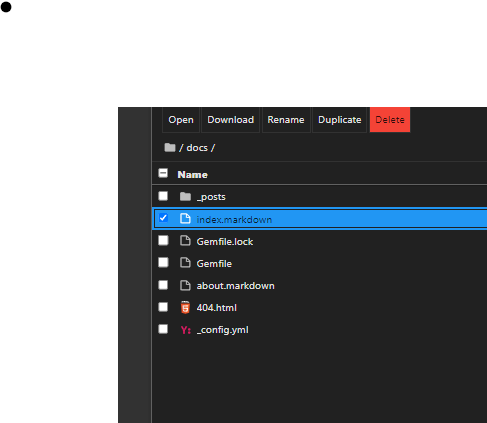
\includegraphics[width=\textwidth]{assets/test.png} % Remplacer par le chemin de l'image
\end{frame}

% Slide 9: Conclusion et Plan d'action
\begin{frame}{Conclusion et Plan d'action}
    \begin{itemize}
        \item \textbf{Modèle final retenu} : LightGBM, avec une AUC de 0.83 et un Score métier de 0.80.
        \item \textbf{Plan d'action pour le déploiement} :
            \begin{itemize}
                \item \textbf{Étape 1} : Déploiement du modèle en production avec un suivi rigoureux des performances.
                \item \textbf{Étape 2} : Mise en place d'un système de mise à jour continue des données pour éviter le concept drift.
                \item \textbf{Étape 3} : Formation des chargés de relation client pour interpréter et expliquer les résultats du modèle.
            \end{itemize}
        \item \textbf{Étapes futures} :
            \begin{itemize}
                \item Amélioration continue du modèle en intégrant des données supplémentaires.
                \item Test de nouvelles techniques de modélisation pour potentiellement améliorer la performance.
            \end{itemize}
    \end{itemize}
\end{frame}

\end{document}
